\documentclass{article}
\usepackage[utf8]{inputenc}
\usepackage{hyperref}
\usepackage{graphicx}
\setlength{\parskip}{1em}
\usepackage[margin=1.0in]{geometry}

\title{Lab 1: Introduction to LabVIEW \\
  \large ECSE 421: Embedded Systems \\ Department of Electrical and Computer Engineering \\ McGill University \\ Version 1.2}
\author{Adam Cavatassi, Jeremy Cooperstock, and Brett Meyer}
\date{Winter 2018}

\begin{document}

\maketitle

\section*{Introduction}
This assignment will serve as your introduction to LabVIEW. Later in the course, you will be
using LabVIEW to program specialized hardware, but for this first assignment you only need
the desktop computers in the lab. In many embedded systems, finite state machines are useful for controlling a program.
Implementing an FSM in LabVIEW is just as easy as in C. In this problem, you will
demonstrate this by writing LabVIEW code to operate a soda machine via FSM. Please read
http://www.ni.com/tutorial/7595/en/ before starting this problem to get an idea about the
implementation.

\section*{Problem}

Suppose you have just invented a new soft drink. You want to sell as much of your product
as possible, but don’t have time to sell it in person because you are too busy working on your
embedded systems project. Since you are an electrical engineer, you decide to build a soda
machine to do the dirty work for you. To compete with Coke and Pepsi, you decide to sell
your sodas for \$0.25 per can. The machine can take nickels, dimes, and quarters. The
machine should dispense a soda as soon as the correct amount is entered. Also, the machine
should be able to make change if someone enters more than \$0.25.

\section*{Designing the FSM}
Design an FSM with 10 states corresponding to each possible value of change that a costumer
enters. Each state has two outputs: the amount of change to be returned to the customer,
and whether or not a soda is dispensed. The state transitions every time the costumer enters
a new coin.
For example, if the user enters a nickel, the FSM will enter the “5 Cents” state. In the “5 Cents”
state, no soda is dispensed, and no change is returned because the total amount entered has not yet reached above \$0.25. From the “5 Cents” state, if the user enters a nickel, the next state will be “10 Cents”; if the user enters a dime, the next state will be “15 Cents”; if the user enters a quarter, the next state will be the "30 Cents" state.



\begin{figure}[h!]
\hspace{15mm} 
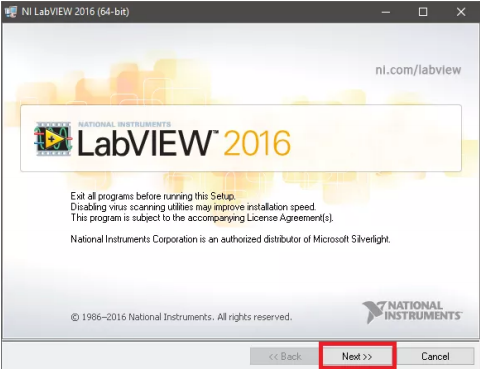
\includegraphics[scale=0.8]{figs/intro.png}
\caption{LabVIEW launch window.}
\label{fig:intro}
\end{figure}

\begin{figure}[h!]
\hspace{18mm} 
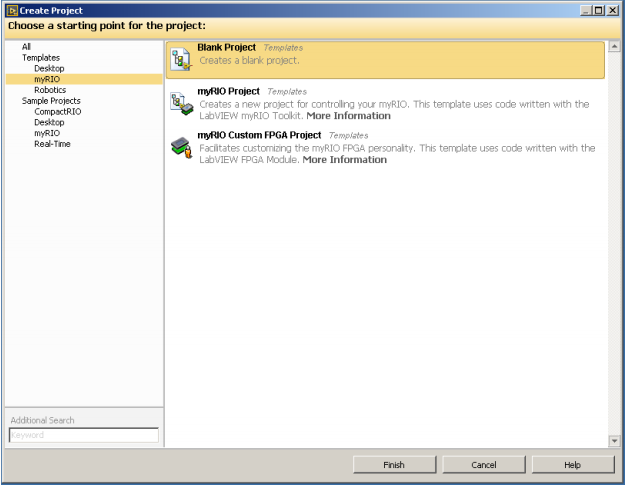
\includegraphics[scale=0.6]{figs/create_project.png}
\caption{Select a blank project.}
\label{fig:create_project}
\end{figure}

\begin{figure}[h!]
\hspace{15mm} 
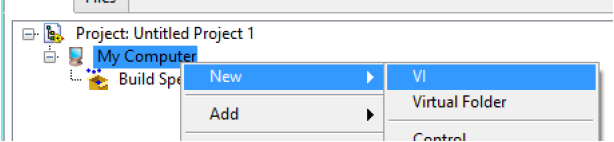
\includegraphics[scale=0.6]{figs/new_vi.png}
\caption{Build a new VI.}
\label{fig:new_vi}
\end{figure}

\section*{Implementing the FSM in LabVIEW}
Now you will implement the FSM you designed in LabVIEW.

\begin{enumerate}
\item Open LabVIEW and click on the \textbf{Create Project} button in the left pane.
\item Select \textbf{Blank Project} and press \textbf{Finish}.
\item In the Project Explorer, right click on \textbf{My Computer}, then \textbf{New}, then \textbf{VI}, to create
a new Virtual Instrument (VI).
\item The front panel and block diagram should then open up. Make a front panel with buttons representing the user entering a nickel, dime, and quarter. There should be a string output for the total change deposited and also the amount of change to be returned. You can use an LED to indicate weather soda has been dispensed or not. Also, use a \textbf{Grab Soda} button to reset the machine after the user has taken his/her soda.
\item Just like in C, an FSM can be implemented as a case structure inside a while loop. The case structure can be found under \textbf{Programming} $\rightarrow$ \textbf{Structures} $\rightarrow$ \textbf{Case Structure}. Place the case structure inside of a while loop. The state can be kept track of using a shift-register (the little up and down arrows at the edge of the while-loop). To get these, right click on the loop boundary and select \textbf{Add Shift Register}. The initial state is piped into the shift register from outside the while-loop. In the code below, an enumeration constant is used so that each state has a unique name. This constant is available on the \textbf{Numeric} palette.
\item Connect the shift register to the little question mark tab on the outside of the case structure. You can add additional cases by right clicking at the case selector on top of the structure and selecting \textbf{Add Case After}.
\item Fill in the logic for each state. It should calculate the next state based on inputs and should calculate the correct outputs as well. You may find the select block useful (\textbf{Programming} $\rightarrow$ \textbf{Comparison} $\rightarrow$ \textbf{Select}). The select block is essentially a multiplexer: the boolean input decides whether to pass the input wired to the true or false terminal.
\end{enumerate}


\begin{figure}[h!]
\hspace{40mm} 
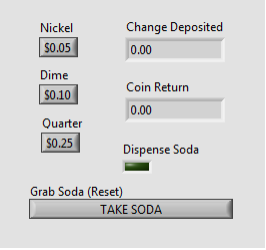
\includegraphics[scale=0.9]{figs/front_panel.png}
\caption{Example front panel of the vending machine VI.}
\label{fig:fp}
\end{figure}

\begin{figure}[h!]
\hspace{-10mm} 
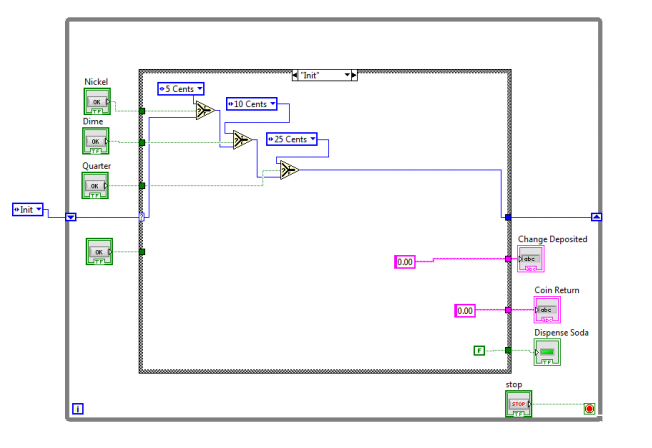
\includegraphics[scale=0.8]{figs/block_diagram.png}
\caption{The VI block diagram.}
\label{fig:bd}
\end{figure}

\begin{figure}[h!]
\hspace{35mm} 
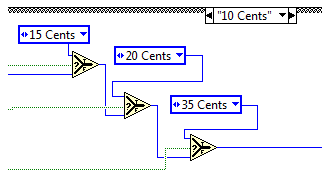
\includegraphics[scale=0.8]{figs/select_block.png}
\caption{Usage of the select block module.}
\label{fig:sb}
\end{figure}

\section*{Submission requirements}

For this lab, you will be required to submit a .zip file containing a screen capture of any one state of the case structure, all your LabVIEW project files, and a README which outlines how to run your code. The README should also include a URL to a private YouTube video with a maximum length of 30 seconds, which illustrates the functionality of your vending machine. Specifically, demonstrate the specific case of inserting a nickel, followed by a dime, followed by a quarter.

\end{document}
